% !TeX root=abs_formeln.tex

\subsection{Ausbreitungsgeschwindigkeit}
\begin{equation}\label{eq:wellen:ausbreitungsgeschwindigkeit}
c = \frac{\lambda}{T} =
\frac{\Delta x}{\Delta t} = \lambda \cdot f
\end{equation}

\subsection{Wellengleichung}
\begin{eqnarray}\label{eq:wellen:gleichung}
s(t,x) &=& \hat{s} \cdot \sin \left[ \omega \left( t - \frac{x}{c} \right)
\right]\\
s(t,x) &=& \hat{s} \cdot \sin \left[ 2\pi \left( \frac{t}{T} - \frac{x}{\lambda}
\right) \right]
\end{eqnarray}

\subsection{Überlagerung von Schwingungen}
\begin{equation}
\begin{split}
\label{eq:schwingung:ueberlagerung}
s(t) &= s_1(t) + s_2(t) \\
&= \hat{s}_1 \cdot \sin(\omega \cdot t) + \hat{s}_2 \cdot
\sin(\omega \cdot t + \varphi_0)
\end{split}
\end{equation}

\subsection{Konstruktive Interferenz}
\begin{equation}
\begin{split}
\label{eq:konstruktive:interferenz}
\Delta \varphi &= 0, 2\pi, 4\pi,\dots\\
 \delta &= k \cdot \lambda, \quad k = 0, 1, 2, \ldots
\end{split}
\end{equation}

\subsection{Destruktive Interferenz}
\begin{equation}
\begin{split}
\label{eq:destruktive:interferenz}
\Delta \varphi &= \pi, 3\pi, 5\pi,\dots \\
 \delta &= (2\cdot k - 1) \cdot \frac{\lambda}{2}, \quad k = 1, 2, 3, \ldots
\end{split}
\end{equation}

\subsection{Verhältnis Gangunterschied zu Phasendifferenz}
\begin{equation}\label{eq:gangunterschied:phasendifferenz}
\frac{\Delta\varphi}{2\pi} = \frac{\Delta s}{\lambda}
\end{equation}

\subsection{Doppler-Effekt}
\subsubsection{Bewegter Beobachter, ruhender Sender}
\paragraph{Annähern}
\begin{equation}\label{eq:doppler:effekt:bewegter:beobachter:annaehern}
f' = f\cdot\left(1 + \frac{v}{c} \right)
\end{equation}

\paragraph{Entfernen}
\begin{equation}\label{eq:doppler:effekt:bewegter:beobachter:entfernen}
f' = f\cdot\left(1 - \frac{v}{c} \right)
\end{equation}

\subsubsection{Bewegter Sender, ruhender Beobachter}
\paragraph{Annähern}
\begin{equation}\label{eq:doppler:effekt:bewegter:sender:annaehern}
\lambda' = \lambda \cdot\left(1 - \frac{v_s}{c} \right) \quad
f' = \frac{f}{1 - \frac{v_s}{c}}
\end{equation}

\paragraph{Entfernen}
\begin{equation}\label{eq:doppler:effekt:bewegter:sender:entfernen}
f' = \frac{f}{1 + \frac{v_s}{c}}
\end{equation}

\subsubsection{Machsche Zahl}
\begin{equation}\label{eq:machsche:zahl}
M = \frac{v_s}{c}
\end{equation}

\subsection{Brechungsgesetz}
\begin{equation}\label{eq:brechungsgestz}
\frac{\sin\alpha}{\sin\beta} = \frac{c_1}{c_2}
\end{equation}

\subsection{Beugung und Interferenz am Doppelspalt}
\begin{center}
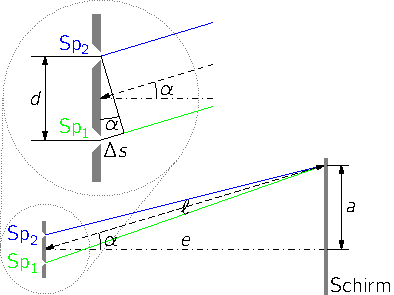
\includegraphics{doppelspalt}
\end{center}
\begin{equation}\label{eq:beugung:doppelspalt}
\sin\alpha = \frac{a}{\ell} = \frac{a}{\sqrt{e^2 + a^2}}
\end{equation}

\subsubsection{Maxima}
\begin{equation}\label{eq:interferenz:doppelspalt:maxima}
n\cdot \lambda = d \cdot \sin \alpha_n
\end{equation}

\subsubsection{Minima}
\begin{equation}\label{eq:interferenz:doppelspalt:minima}
(2\cdot n - 1) \cdot \frac{\lambda}{2} = d \cdot \sin \alpha_n
\end{equation}

\subsection{Beugung und Interferenz am Gitter}
\begin{equation}\label{eq:beugung:gitter}
n \cdot \lambda = g \cdot \sin\alpha_n = \frac{g \cdot a_n}{\ell} =
\frac{g \cdot a_n}{\sqrt{e^2 + a_n^2}}
\end{equation}
